\section{Organization \& conduct of the meeting}

The \symp will be organized in many ways traditionally and others
not. The key idea at this event is to engage in ways that are direct and
across well-entrenched disciplinary and geographic lines. And to do so,
in ways that can shape nascent ideas that a speaker might want to
present and one that might not have been whetted before. Second, we
expect speakers to engage not their typical trusted peers, but those
well outside their nominal comfort zone. This does two things; one to
articulate an idea/concept in ways that is accessible and
jargon-free. And two, it forces the ideation process to bridge divides
that tend to persist in typical siloed academic settings.

We will do so, by asking every speaker to think about technology -- if
they're scientists. And to think science if they're technologists. So
for instance, if a technologist talks about making water-column
measurements, we would expect the challenger (and the audience in turn)
to poke and prod the speaker away from traditional straight-line
transects. That could (potentially) lead to discussion on sampling
strategies (and Sampling Theory), and in turn (and hopefully) drive the
speaker to a more curiosity driven approach to why and how the biology
(say) does what it does. This also means that a pre-requisite to
accepting the invitation, a participant has to commit to doing work
\emph{prior} to the meeting, to ideate the concept in accessible
ways. And to engage the assigned challenger via any form of
communication (Video, audio calls, email e.t.c) so they can understand
and approach the problem in their own individual ways. We expect the
pairing of the speaker with a challenger to occur about 2 months prior
to the event, ensuring sufficient time for the participants to interact
with one another and come prepared with their own notions of the ideated
concept and its potential critique. 

At the meeting, each speaker will present her/his idea and be
'challenged' by the other. Audience participation will be crucial, so as
to ensure that the concept(s) is exposed to more diverse opinion, yet
driven by the speaker and the challengers critique. To instantiate this,
we will hold the following structure to each talk.

\begin{itemize}[noitemsep,topsep=0pt,parsep=0pt,partopsep=0pt]

\item 20 minutes -- Speaker presentation in some measure of
  detail and accessible to the audience
\item 10 minutes -- Commentator, providing
  feedback/critique/comments/suggestions
\item 5 minutes -- Speaker response/rebuttal

\end{itemize}


\begin{figure}[!h]
  \centering 
  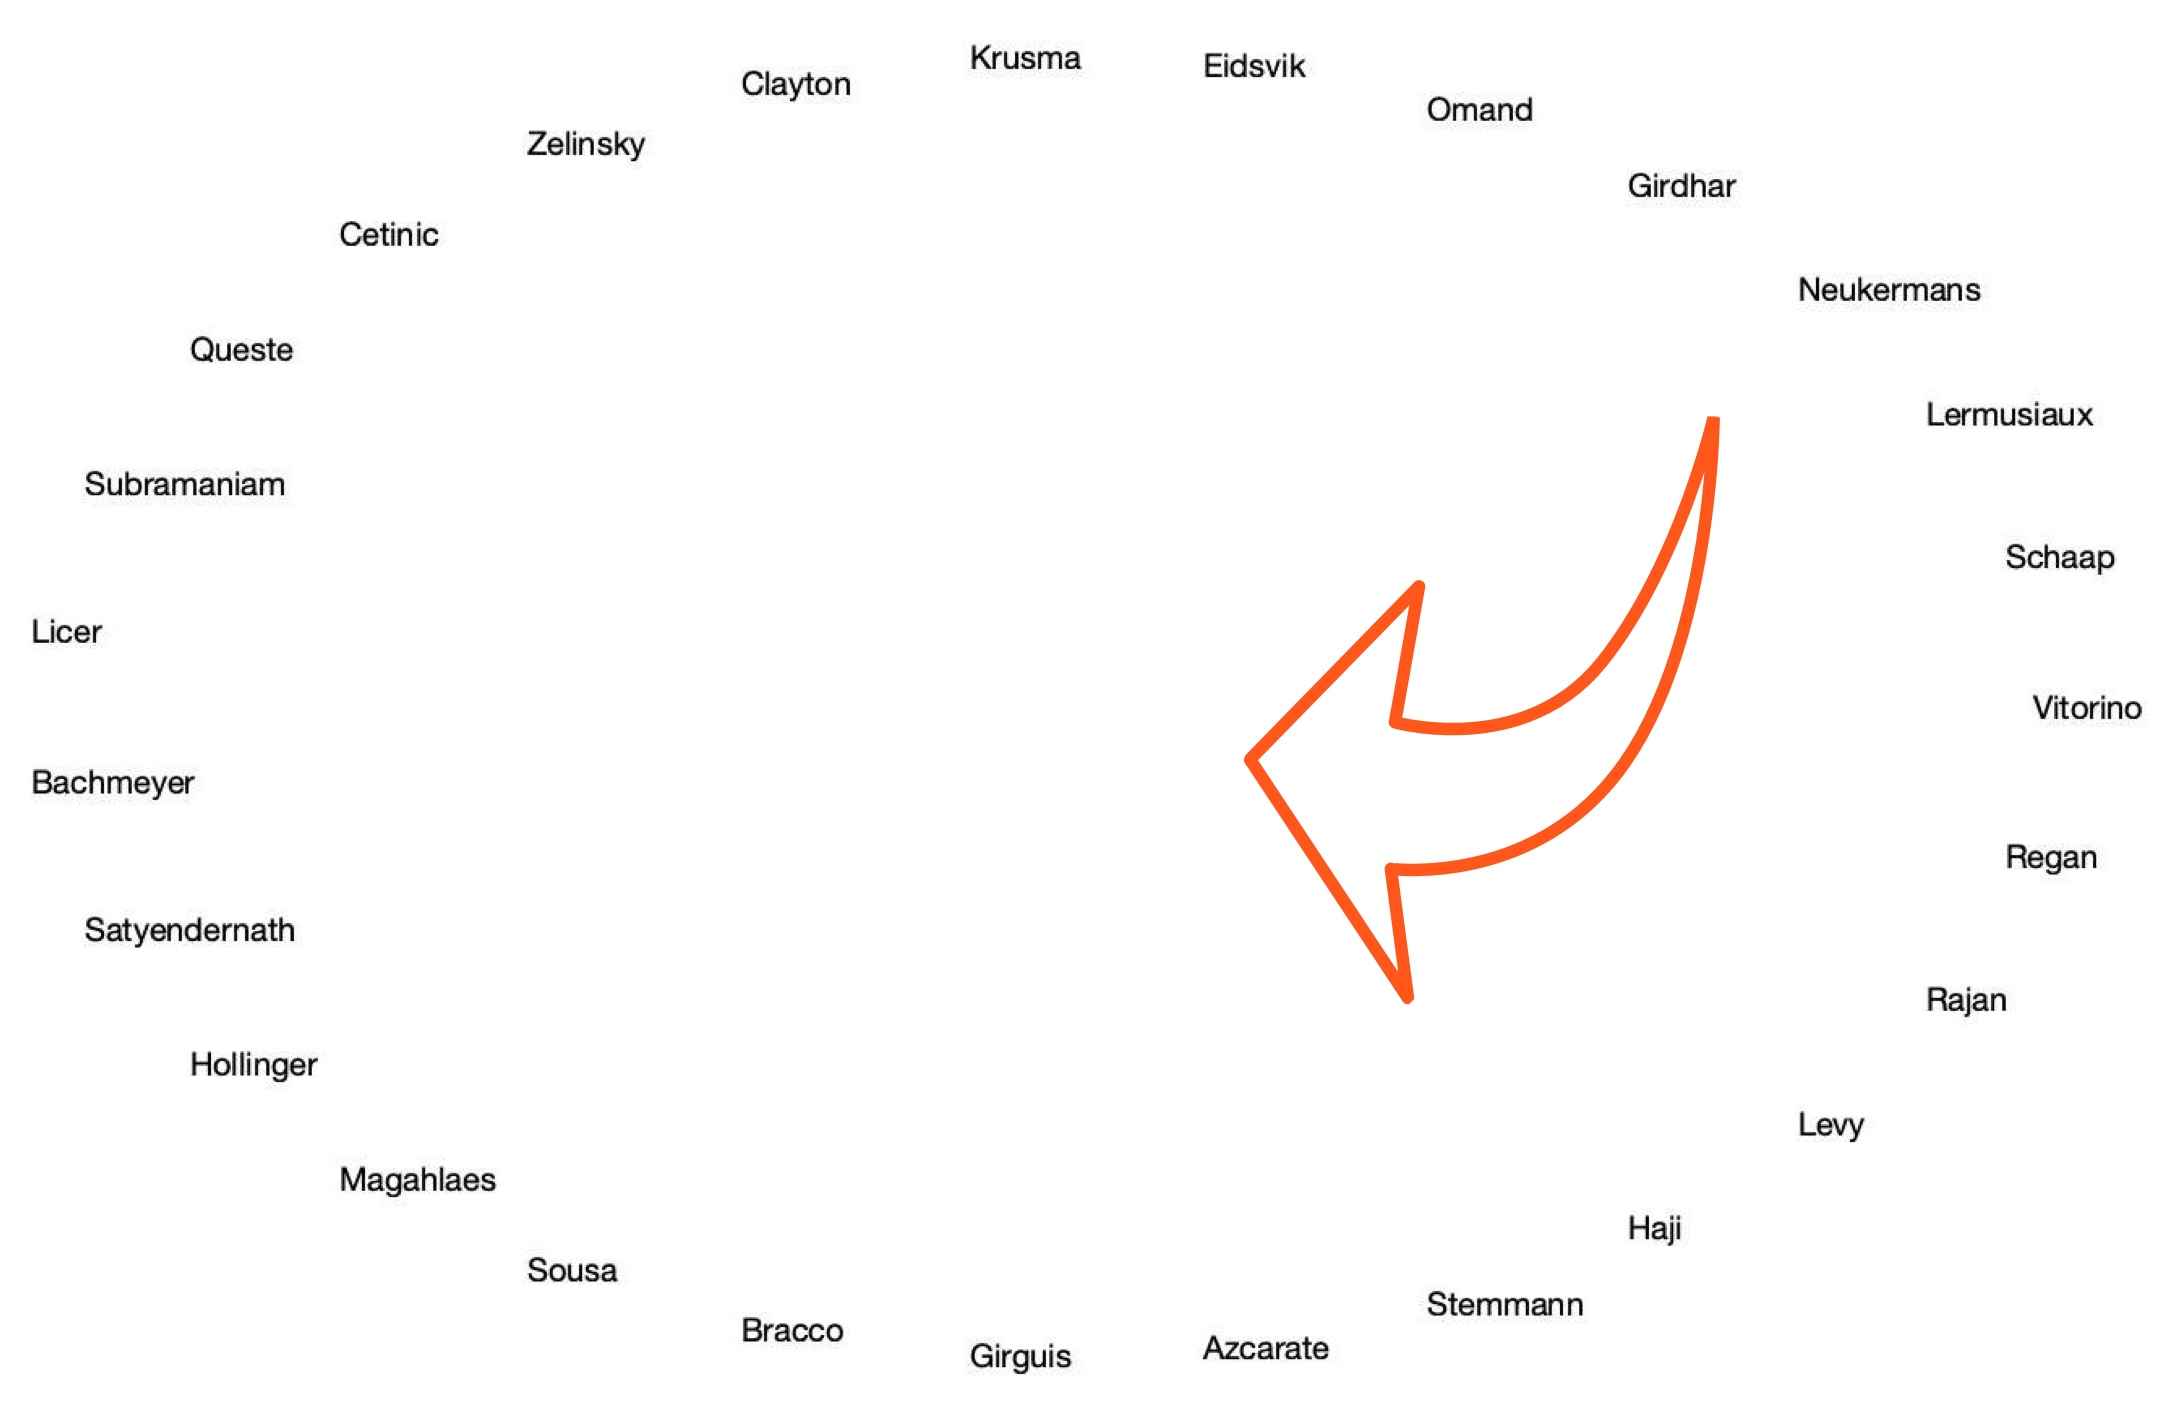
\includegraphics[scale=0.15]{fig/pairing.jpg}
  \caption{A example pairing of participants. Each person sends
    his/her presentation material to the connected person in the
    clockwise direction, while receiving material from the other
    connection.}
  \label{fig:pairs}
\end{figure}

A preliminary proposal of the pairing is shown in
Fig. \ref{fig:pairs}, with each participant paired with two others,
one as a speaker, the other as a critique for a different speaker. As
shown, a presenter sends her/his inputs in the clockwise direction,
while the critique/commentator provides feedback in the anti-clockwise
direction.  The pairing is constructed to maximize the variety in the
workshop topics, while keeping some scientific element in common
within each pair. Notably, our algorithm also attempts to spread the
gender, continent and seniority level in pairs. Our goal with this is
to faciliate a constructive discussion among participants that can
also spark new ideas in this multidisciplinary setting.

\subsection{Timeline of events}

The following are the timeline of events, consistent with the ongoing
planning for the symposium.

\begin{figure}[!h]
  \centering 
  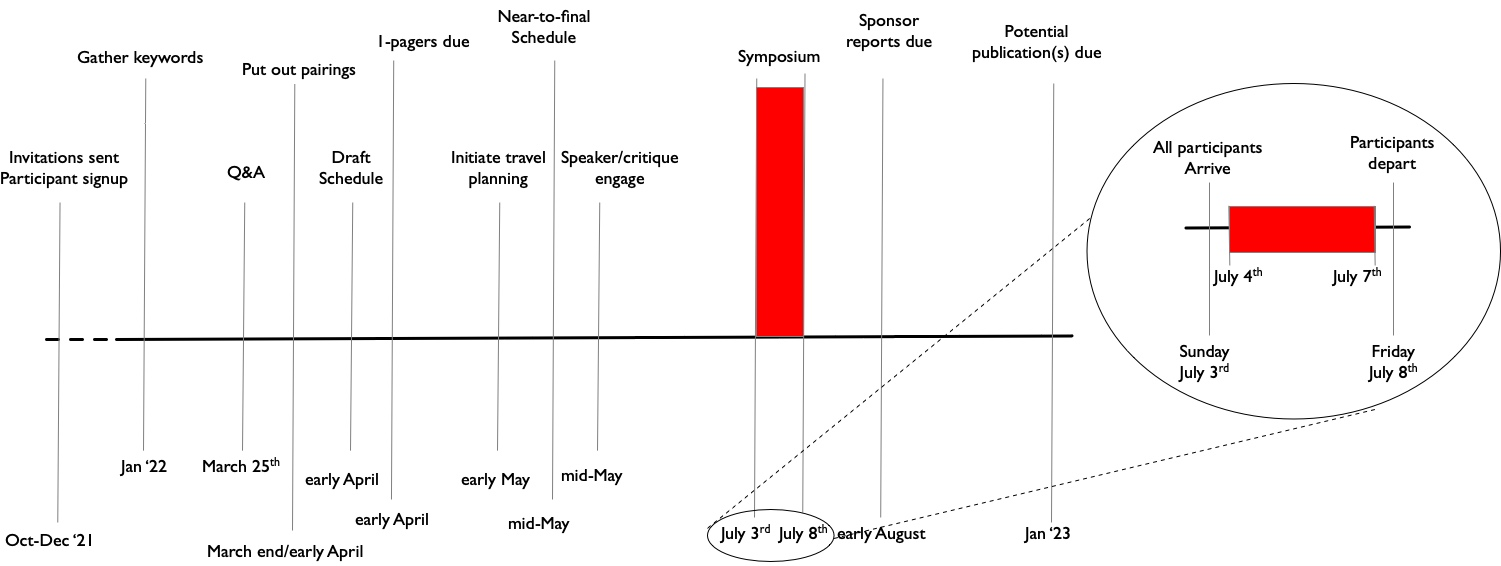
\includegraphics[scale=0.3]{fig/timeline.jpg}
  \caption{The timeline of events leading to and beyond the symposium
    in July 2022 which has been shared with all participants.}
  \label{fig:timeline}
\end{figure}
